\rewrite{INICIO - sobre AFD baseado em atributos vs baseado em exemplos}

\rewrite{
No âmbito de AFD podemos identificar duas abordagens distintas: baseado em exemplos e baseado em atributo.

As técnicas de AFD baseado em atributos consideram um conjunto de múltiplos FD e o objetivo do aprendizado é identificar padrões de comportamento entre os diferentes conjuntos. A \autoref{Fig:AgrupMultiStream} apresenta um \emph{framework} popular para o agrupamento de múltiplos FD. Os FDs de entrada são gerenciados por um mecanismo que mantém uma sumarização estatística dos fluxos e é capaz de realizar uma partição dos múltiplos FDs pela análise de métricas que comparem os atributos presentes no fluxo. Um exemplo seria o agrupamento do histórico de diferentes ações da bolsa de valores, associando ações com tendências semelhantes a um mesmo grupo.

\begin{figure}[!htb]
	\centering
	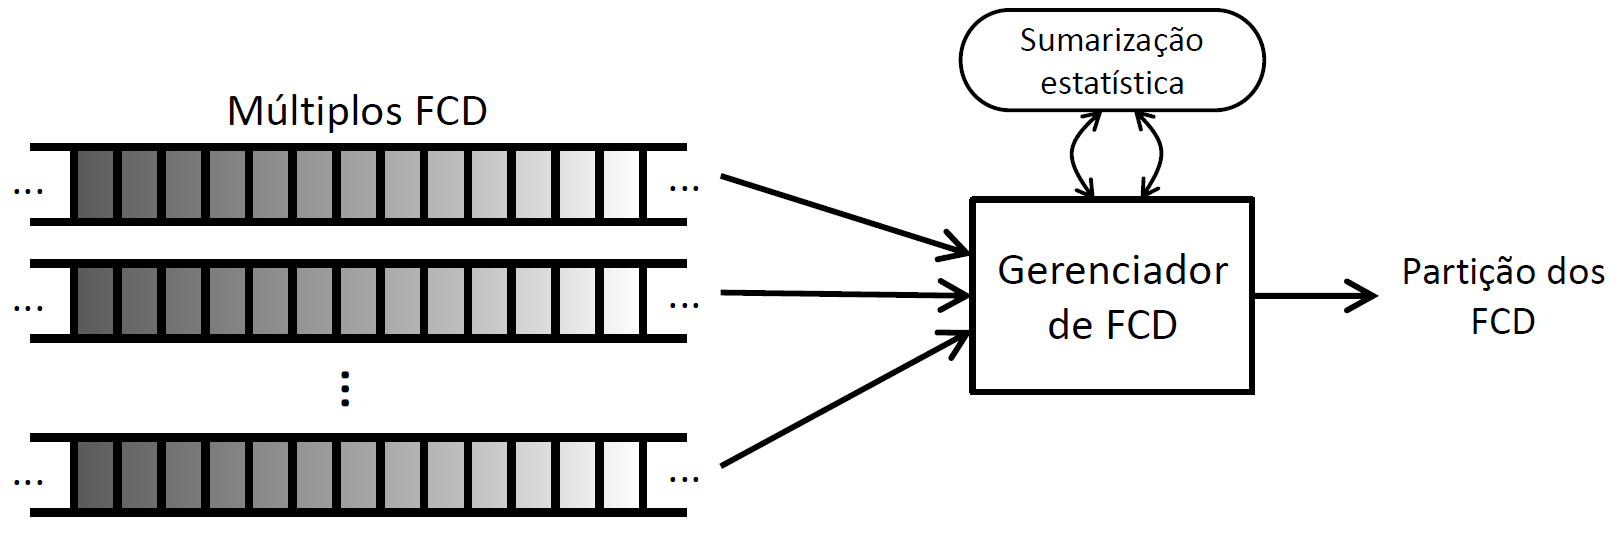
\includegraphics[width=0.7\textwidth]{figures/multiStream}
	\caption{\rewrite{modificar a figura, se for mantida}\emph{Framework} para agrupamento baseado em atributo (múltiplos FD) \cite{Silva2013}}\label{Fig:AgrupMultiStream}
\end{figure}

Estratégias de aprendizado supervisionado de múltiplos FD seguem esquema similar, porém considerando a informação de rótulo de cada fluxo como objetivo do aprendizado. O aprendizado semissupervisionado surge como parte de esforços para a proposta de mecanismos capazes de aprender a partir de múltiplos FDs.

\citeonline{Chen2013} propõem uma estrutura de sumarização para a representação de exemplos de FDs de forma compacta com o objetivo de agrupar múltiplos FDs de forma não supervisionada. O algoritmo \emph{MINETRAC} \cite{Casas2011} combina técnicas de aprendizado não supervisionado e semissupervisionado para identificação e classificação de diferentes classes de fluxos de tráfego de internet, que possuam características similares. Um método semissupervisionado baseado em grafo \cite{Li2014} para propagação de rótulos e extensão do conjunto rotulado que realiza o treinamento de um classificador usando \emph{Support Vector Machine} é utilizado para a identificação de padrões em sequências de dados.

As técnicas que seguem a abordagem de aprendizado baseado em exemplos tem como objetivo criar um modelo correspondente aos dados de um FD único.}

\rewrite{FIM - sobre AFD baseado em atributos vs baseado em exemplos}